% fancytikzposter.tex, version 2.1
% Original template created by Elena Botoeva [botoeva@inf.unibz.it], June 2012
% 
% This file is distributed under the Creative Commons Attribution-NonCommercial 2.0
% Generic (CC BY-NC 2.0) license
% http://creativecommons.org/licenses/by-nc/2.0/ 


\documentclass{a0poster}

\usepackage{fancytikzposter} 


%%%%% --------- Change here if you want ---------- %%%%%
%% margin for the geometry package, must be changed before using the geometry package
%% default value is 4cm
% \setmargin{4}

%% the space between the blocks
%% default value is 2cm
% \setblockspacing{2}

%% the height of the title stripe in block nodes, decrease it to save space
%% default value is 3cm
% \setblocktitleheight{3}

%% the number of columns in the poster, possible values 2,3
%% default value is 2
% \setcolumnnumber{3}

%% the space between two or more groups of authors from different institutions
%% used in \maketitle
% \setinstituteshift{10}

%% which template to use
%% N1 simple, standard look, with a colored background and gray boxes
%% N2 board with nodes
%% N3 another standard look
%% N4 envelope-like look
%% N5 with a wave-like head, original idea taken from
%%%% http://fc09.deviantart.net/fs71/f/2010/322/1/1/scientific_poster_by_nabuy-d333ria.jpg
\usetemplate{2}

%% components of the templates
%% (the maximal possible numbers are mentioned as the parameters)
% \usecolortemplate{4}
% \usebackgroundtemplate{5}
% \usetitletemplate{2}
% \useblocknodetemplate{5}
% \useplainblocktemplate{4}
% \useinnerblocktemplate{2}


%% the height of the head drawing on top 
%% applicable to templates N3, 4 and 5
% \setheaddrawingheight{14}


%% change the basic colors
%\definecolor{myblue}{HTML}{008888} 
%\setfirstcolor{myblue}% default 116699
%\setsecondcolor{gray!80!}% default CCCCCC
%\setthirdcolor{red!80!black}% default 991111

%% change the more specific colors
% \setbackgrounddarkcolor{colorone!70!black}
% \setbackgroundlightcolor{colorone!70!}
% \settitletextcolor{textcolor}
% \settitlefillcolor{white}
% \settitledrawcolor{colortwo}
% \setblocktextcolor{textcolor}
% \setblockfillcolor{white}
% \setblocktitletextcolor{colorone}
% \setblocktitlefillcolor{colortwo} %the color of the border
% \setplainblocktextcolor{textcolor}
% \setplainblockfillcolor{colorthree!40!}
% \setplainblocktitletextcolor{textcolor}
% \setplainblocktitlefillcolor{colorthree!60!}
% \setinnerblocktextcolor{textcolor}
% \setinnerblockfillcolor{white}
% \setinnerblocktitletextcolor{white}
% \setinnerblocktitlefillcolor{colorthree}




%%% size of the document and the margins
%% A0
% \usepackage[margin=\margin cm, paperwidth=118.9cm, paperheight=84.1cm]{geometry} 
\usepackage[margin=\margin cm, paperwidth=84.1cm, paperheight=118.9cm]{geometry}
%% B1
% \usepackage[margin=\margin cm, paperwidth=70cm, paperheight=100cm]{geometry}



%% changing the fonts
\usepackage{cmbright}
%\usepackage[default]{cantarell}
%\usepackage{avant}
%\usepackage[math]{iwona}
\usepackage[math]{kurier}
\usepackage[T1]{fontenc}


%% add your packages here
\usepackage{hyperref}
\usepackage[utf8]{inputenc} % slovenski znaki
\usepackage[slovene]{babel} % slovenski formati
\usetikzlibrary{shapes,arrows}

\title{Letter classification}
\author{Rok Koleša, Domen Kren, Darko Janković\\
  Faculty of Computer and Information science, University of Ljubljana
}


\begin{document}

%%%%% ---------- the background picture ---------- %%%%%
%% to change it modify the macro \BackgroundPicture
\ClearShipoutPicture
\AddToShipoutPicture{\BackgroundPicture}

\noindent % to have the picture right in the center
\begin{tikzpicture}
  \initializesizeandshifts
  % \setxshift{15}
  % \setyshift{2}


  %% the title block, #1 - shift, the default value is (0,0), #2 - width, #3 - scale
  %% the alias of the title block is `title', so we can refer to its boundaries later
  \ifthenelse{\equal{\template}{1}}{ 
    \titleblock{47}{1}
  }{
    \titleblock{47}{1.5}
  }

  %% a logo can be added to the title block
  %% #1 - anchor relative to the title block, #2 - shift, #3 - width, #3 - file name
  % \ifthenelse{\equal{\template}{2}}{ 
  %   \addlogo[south west]{(2,0)}{6cm}{unibz_b.png}
  % }{
  %   \addlogo[south west]{(2,0)}{6cm}{unibz_w.png}
  % }


  %% a block node, with the specified position (optional), title and the content
  %% #1 - where (optional), #2 - title, #3 - text
  %%%%%%%%%% ------------------------------------------ %%%%%%%%%%
  \blocknode%
  {Problem}%
  {
  \coloredbox{colorthree!50!}{
  Determine which capital letter is represented by given simplicial complex from the set of 12 letters of Slovenian alphabet. Simplicial complex is represented with a list of edges which consist of pairs of start and end points. Each point is given by a pair of coordinates.}
  }
  
 
  
  \blocknode{Sinking example}
  {
  \setlength{\tabcolsep}{40pt}
  \begin{tabular}{c c c}
      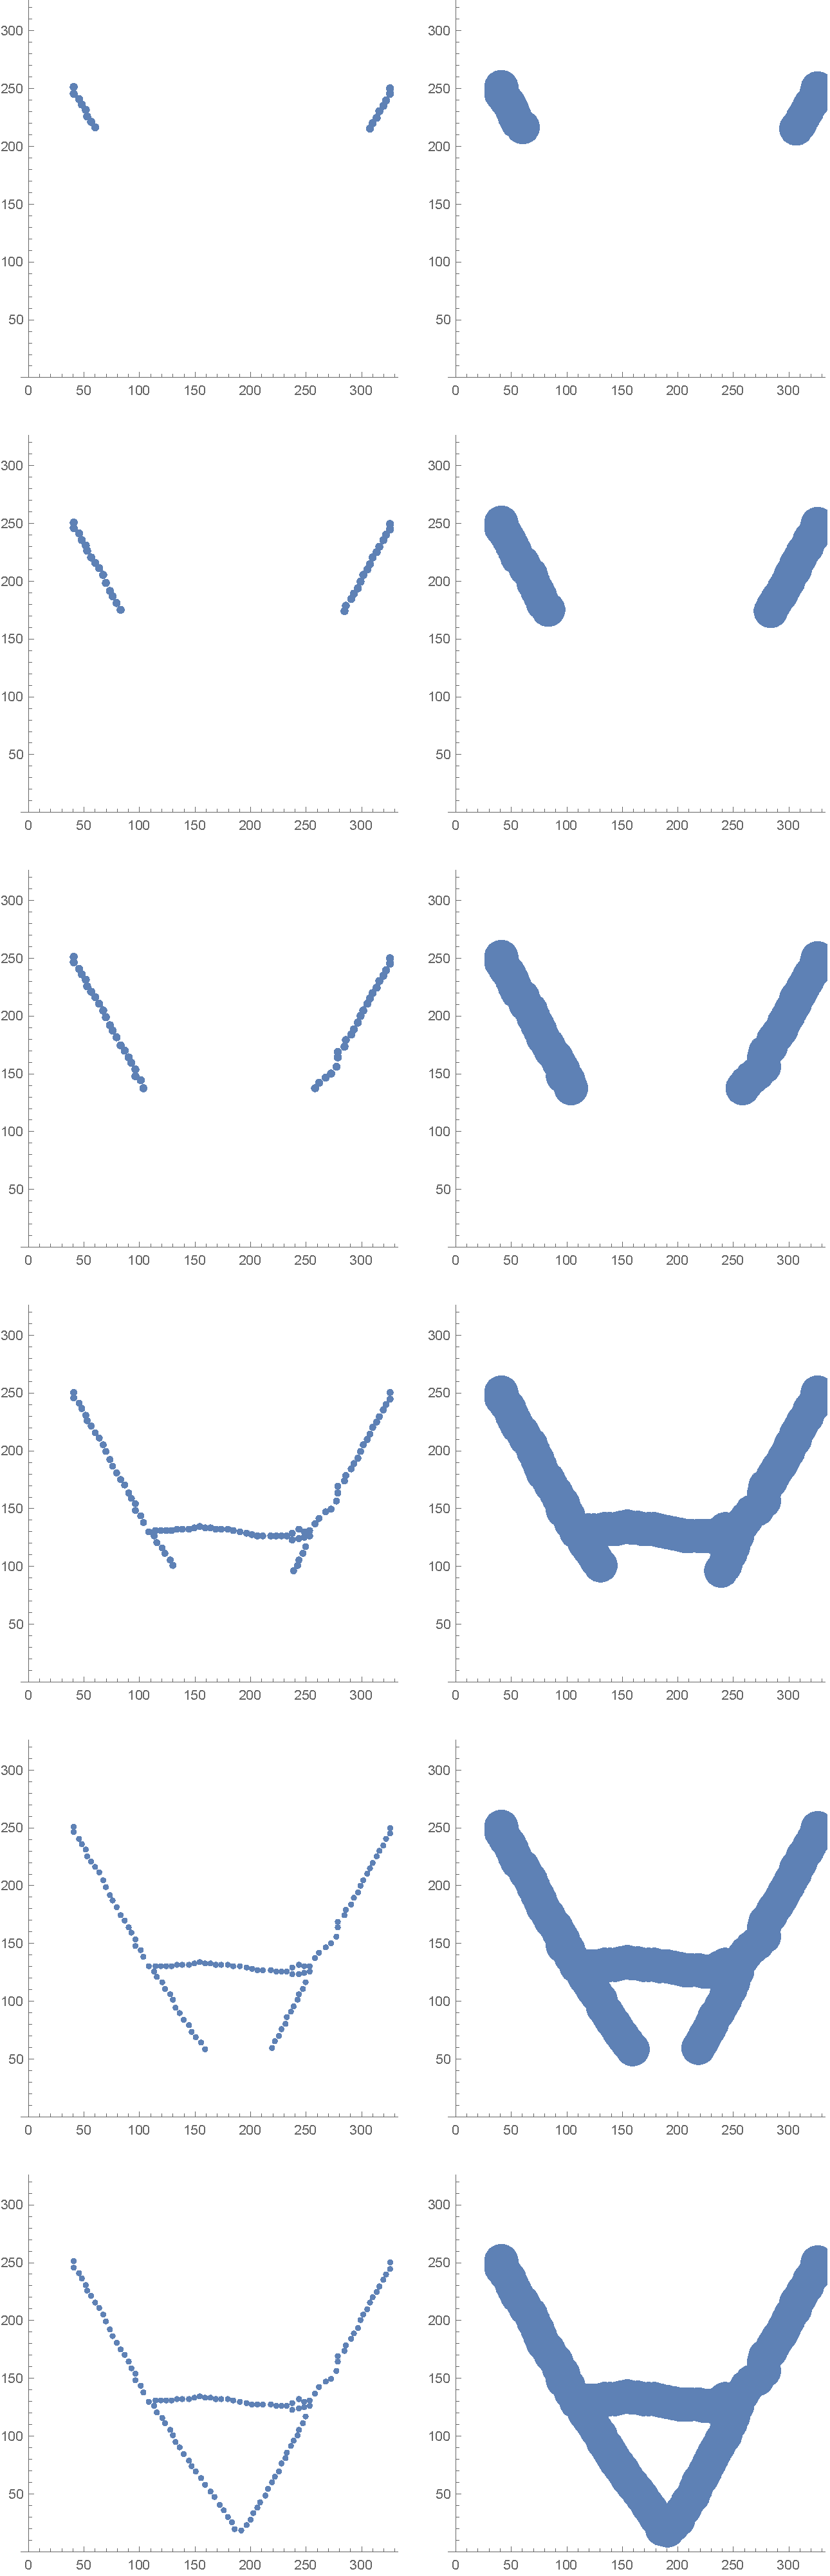
\includegraphics[scale=0.4]{../images/RT-A-cuts.pdf}
      &
      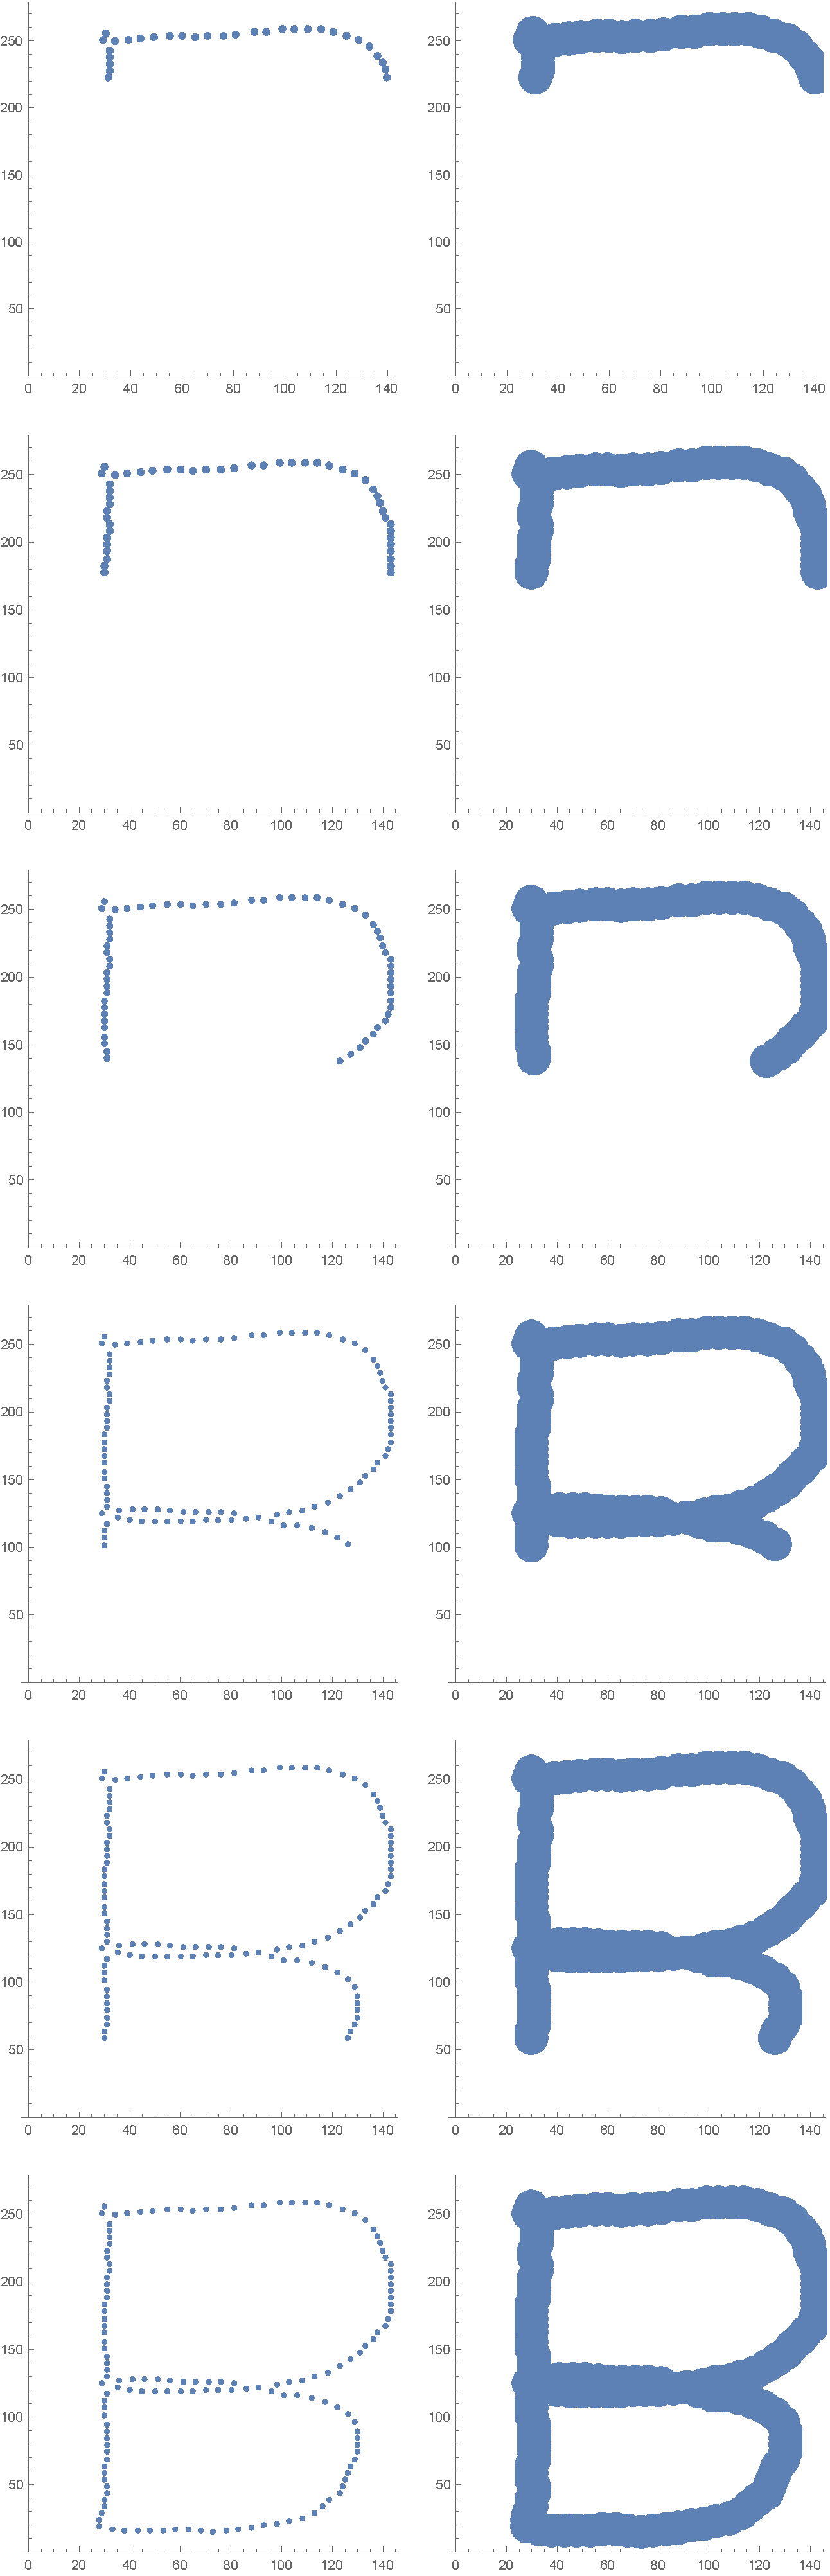
\includegraphics[scale=0.4]{../images/RT-B-cuts.pdf}
      &
      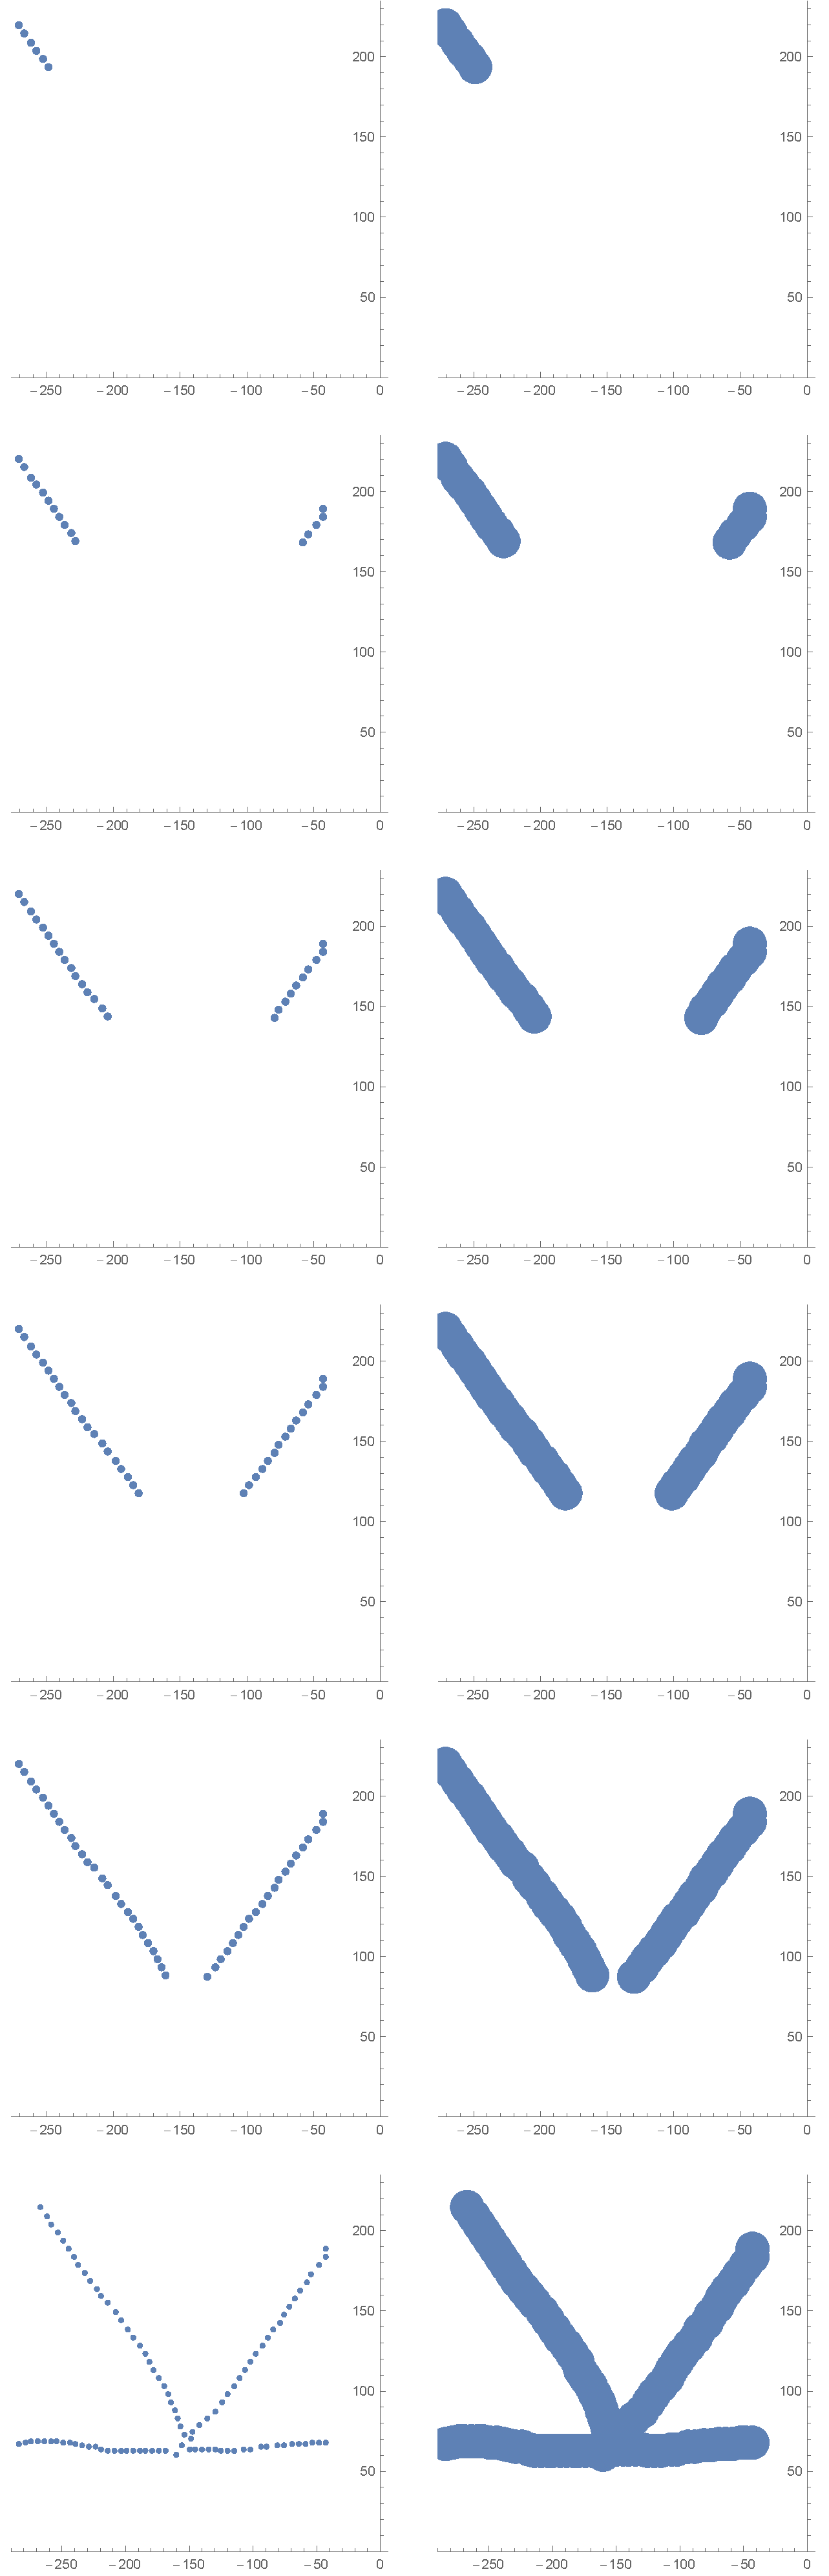
\includegraphics[scale=0.4]{../images/RT-K-90-cuts.pdf}\\
      
      \multicolumn{3}{c}{Fig 2: Sinking of letters A, B and K (rotated for 90 degrees)}

  \end{tabular}
    
  
  }
  
  \blocknode{Betti numbers by cuts}
  {
  \setlength{\tabcolsep}{0pt}
  \begin{tabular}{c c}
        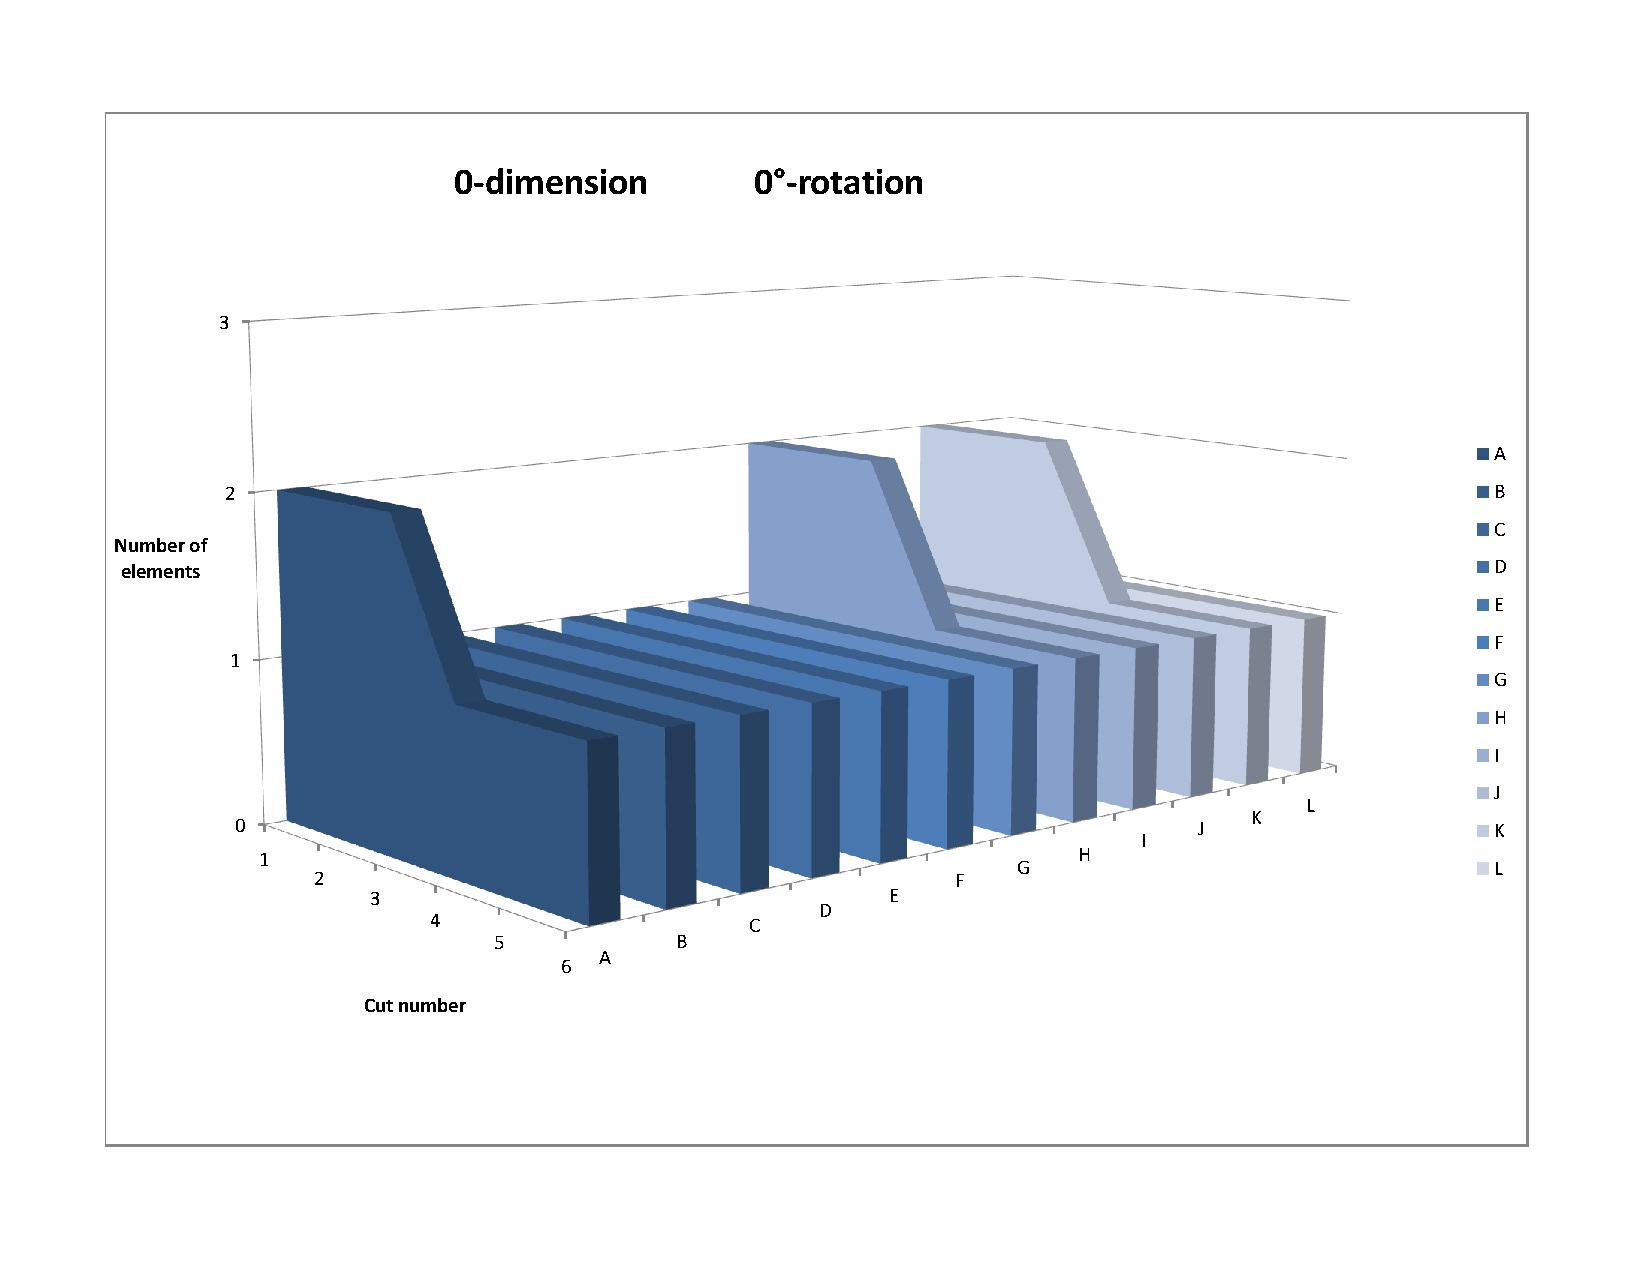
\includegraphics[scale=0.6]{../images/0D_0deg.pdf}
        &
        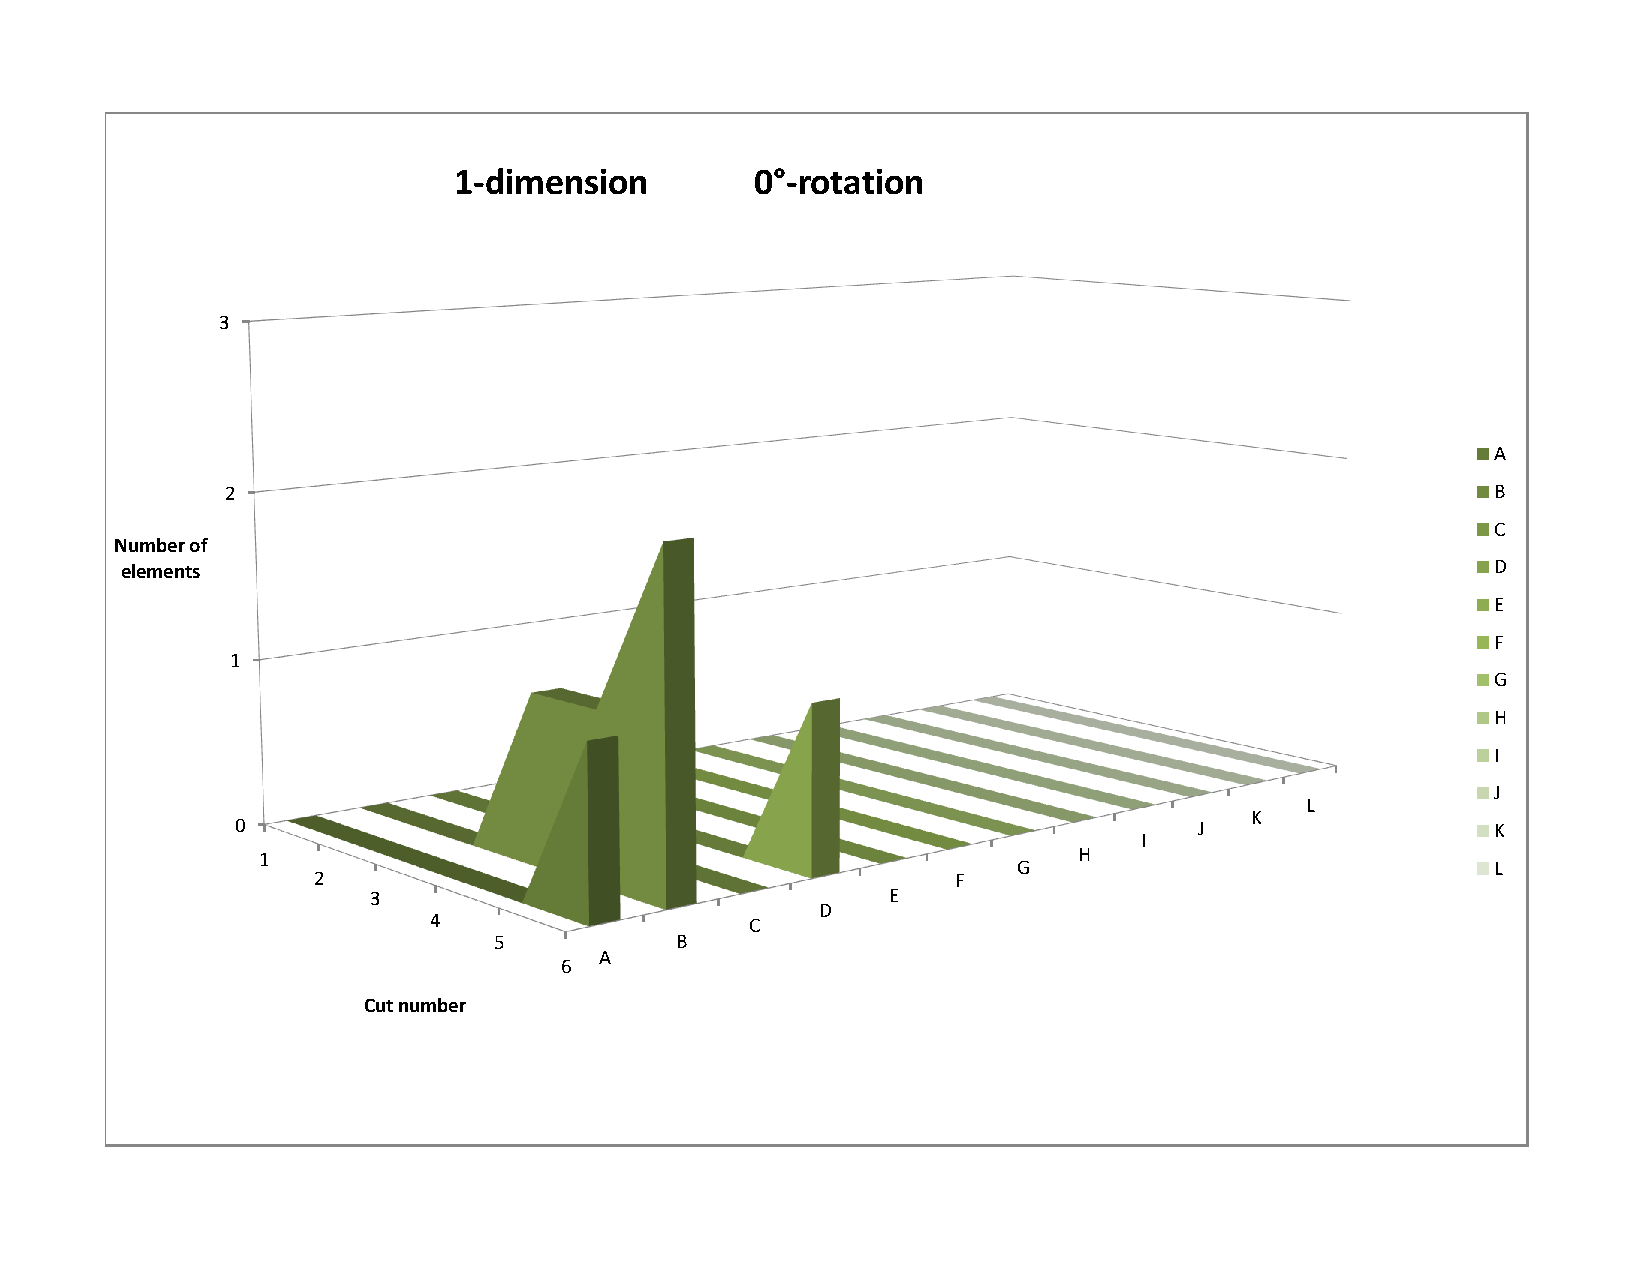
\includegraphics[scale=0.6]{../images/1D_0deg.pdf}\\
        \multicolumn{2}{c}{Fig 3: Betti numbers for dimensions 0 and 1, no rotation}
  
  \end{tabular}
  
  
  
  }
%%%%%%%%%% ------------------------------------------ %%%%%%%%%%

  
  


  %%%%%%%%%%%%% NEW COLUMN %%%%%%%%%%%%%%% 
  \startsecondcolumn 

  %%%%%%%%%% ------------------------------------------ %%%%%%%%%%
  \blocknode%
  {Solution}%
  {

As seen in our goal specification, we tackled this problem of letter classification with persistent homology. 
The main idea of our solution is looking at different parts of objects and computing their homologies. The 
algorithm is divided into three parts:

\begin{enumerate}
\item First, let us parse the input. All we need is a set of points that are part of the object we want to classify. The
only problem that can arise, comes from the distribution of the points. If they are all in one place or to scarce, we
will not be able to get good results. We want an even distribution with lots of points.

\item We slowly ''sink'' our letter. After sorting our input points we cut the letter by layers. After that we compute 
homologies for each of those. 

For the computations, we use the VietorisRips filter and check the intervals of our 
simplexes. In this case, we take the infinite ones. With that we can get the number of pieces and cycles in our complex.
We have to be a little careful with how we chose the maximum radius value, for the VietorisRips algorithm. With some
trial and error we decided on 10\% of the full object size. With that we remove most of errors. 

Now let us return to the ''sinking''. For example, lets break letter ''A'' into 6 pieces. First, we take the lowest piece and 
get its 0. and 1. dimension homologies. The next step is the lowest two pieces, then three, ... What we get in the end is 
a diagram with numbers corresponding to the number of pieces and cycles for every part of the letter.

\item The last thing we need to do is classify the letter. Based on some observations we made a decision tree, which ''sinks''
the given letter in many directions and based on the observations chooses the correct paths. For example, in the first
stage we look at the number of cycles in the letter. Based on that information we can already separate "B" from the others, as
it is the only one with 2. With this information can also separate ''A'' and ''D'' from all the others. Every group of potential
candidates can be separated with different information (we ''sink'' top to bottom, left to right, 45 degree angle, ...) until we
are left with only one candidate in each node. This candidate corresponds to our original letter so we return it. 

\end{enumerate}

}

  \blocknode{Decision tree}{
    \begin{tikzfigure}[Letter decision tree]
        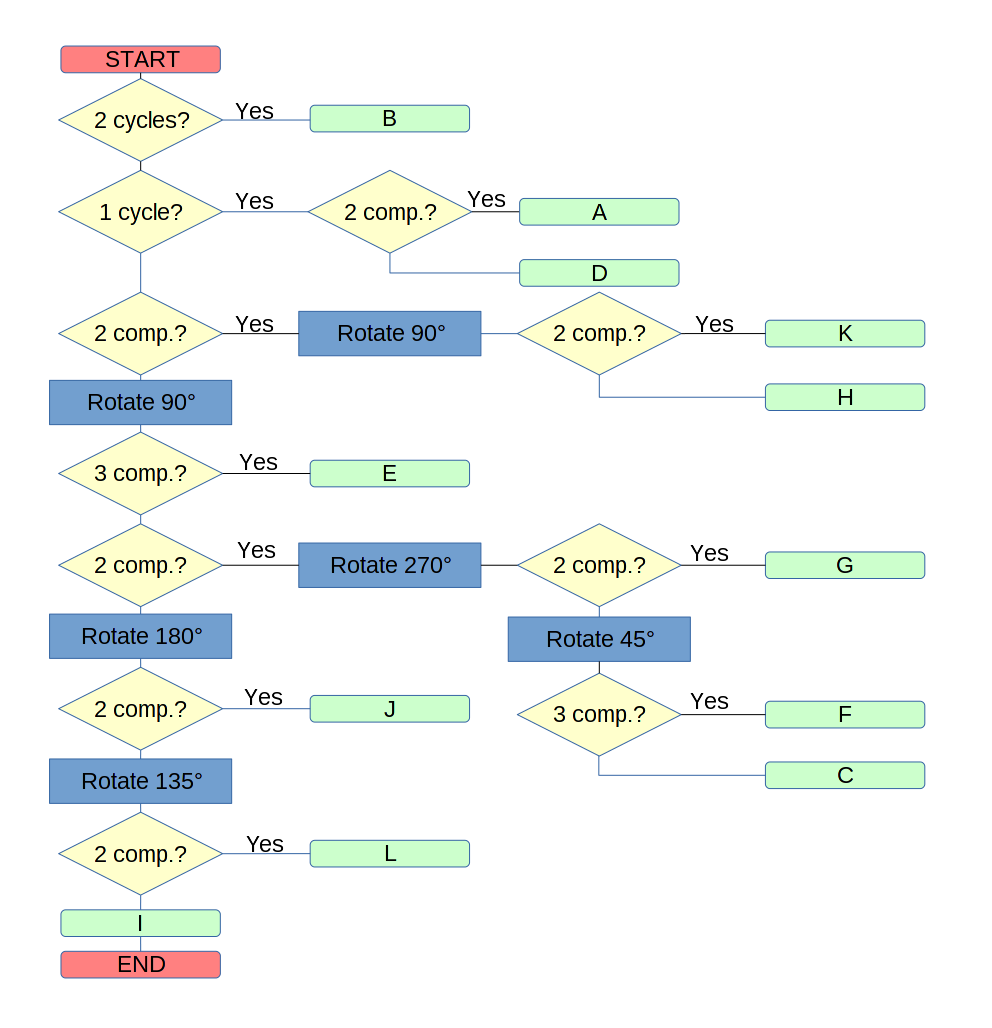
\includegraphics[scale=0.8]{../images/DecisionTree.png}
    \end{tikzfigure}
  }
    
  \blocknode{Results}%
  {With described method we were able to successfully classify input data.  

  }
  





\end{tikzpicture}


\end{document}




